\begin{minipage}[c]{\textwidth}
\advance\leftskip-2.5cm
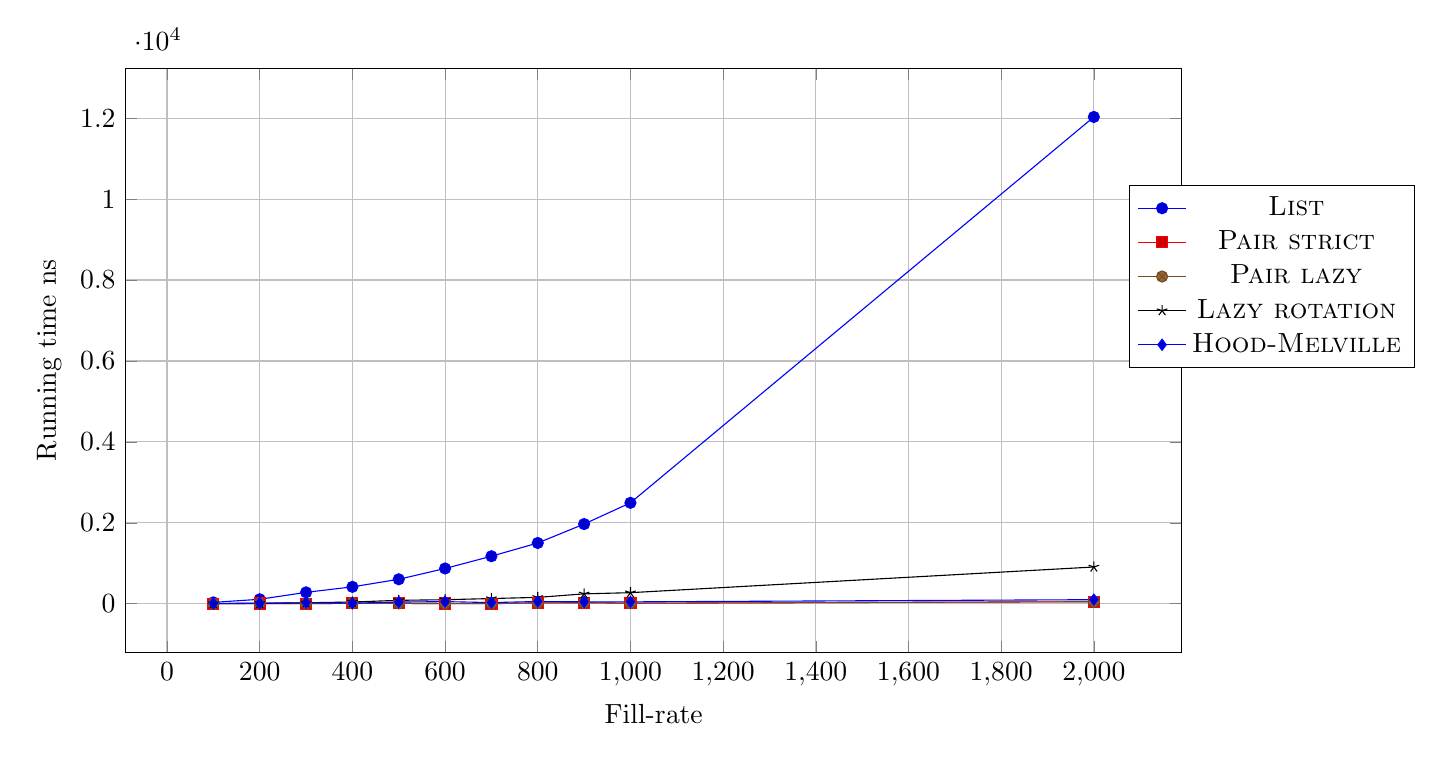
\begin{tikzpicture}
        \begin{axis}[
            xlabel = Fill-rate,
            ylabel = Running time ns,
            height=9cm,
            width=15cm,
            grid=major,
            legend style={
            at={(0.95,0.8)},
            anchor=north west}]            
            legend pos=center west
    	]
    		
    		
    	\addplot coordinates {
(100,33)
(200,110)
(300,281)
(400,417)
(500,604)
(600,871)
(700,1174)
(800,1501)
(900,1969)
(1000,2494)
(2000,12031)

    	};
        
    	\addlegendentry{\textsc{List}}

                \addplot coordinates {
(100,0)
(200,5)
(300,3)
(400,10)
(500,8)
(600,4)
(700,3)
(800,20)
(900,26)
(1000,12)
(2000,50)

    	};
        
    	\addlegendentry{\textsc{Pair strict}}

        \addplot coordinates {
(100,0)
(200,5)
(300,3)
(400,10)
(500,8)
(600,4)
(700,3)
(800,20)
(900,26)
(1000,12)
(2000,50)

    	};
        
    	\addlegendentry{\textsc{Pair lazy}}

        \addplot coordinates {
(100,2)
(200,9)
(300,24)
(400,42)
(500,84)
(600,99)
(700,128)
(800,157)
(900,244)
(1000,273)
(2000,908)

    	};
        
    	\addlegendentry{\textsc{Lazy rotation}}

        \addplot coordinates {
(100,8)
(200,13)
(300,24)
(400,14)
(500,41)
(600,52)
(700,28)
(800,55)
(900,47)
(1000,46)
(2000,100)

    	};
        
    	\addlegendentry{\textsc{Hood-Melville}}

        \end{axis}

    \end{tikzpicture}
    \captionof{figure}{TITEL}
    \label{fig:sample_figure}
\end{minipage}